\documentclass{article}
\usepackage{graphicx}
\usepackage{amsmath}
\usepackage{hyperref}
\usepackage{listings}
\usepackage{float}

\usepackage{color}
\definecolor{lightgray}{rgb}{.9,.9,.9}
\definecolor{darkgray}{rgb}{.4,.4,.4}
\definecolor{purple}{rgb}{0.65, 0.12, 0.82}

\lstdefinelanguage{JavaScript}{
  keywords={typeof, new, true, false, catch, function, return, null, catch, switch, var, if, in, while, do, else, case, break},
  keywordstyle=\color{blue}\bfseries,
  ndkeywords={class, export, boolean, throw, implements, import, this},
  ndkeywordstyle=\color{darkgray}\bfseries,
  identifierstyle=\color{black},
  sensitive=false,
  comment=[l]{//},
  morecomment=[s]{/*}{*/},
  commentstyle=\color{purple}\ttfamily,
  stringstyle=\color{red}\ttfamily,
  morestring=[b]',
  morestring=[b]"
}

\lstset{
   language=JavaScript,
   backgroundcolor=\color{lightgray},
   extendedchars=true,
   basicstyle=\footnotesize\ttfamily,
   showstringspaces=false,
   showspaces=false,
   numbers=left,
   numberstyle=\footnotesize,
   numbersep=9pt,
   tabsize=2,
   breaklines=true,
   showtabs=false,
   captionpos=b
}

\title{%
Howework 2 \\
\large Interactive Graphics}

\date{June 2018}
\author{Ibis Prevedello}

\begin{document}
\maketitle

\section{Introduction}
The goal of this homework is to use WebGL with control code written in JavaScript in order to draw an interactive 3D dog in an HTML canvas in a web browser. The source code for this project can be accessed from my \href{https://github.com/ibiscp/Computer-Graphics-WebGL/tree/master/Homework2}{GitHub page}.

\section{Development}
A series of improvements were implemented in the base code in order to achieve the following effects:

\begin{enumerate}
\item Create a hierarchical model of a (simplified) dog, composed of the body, 4 legs (each one composed of 2 independent components, upper and lower leg), head and tail. All components are cubes, use the cube function present in the file
\item Add a procedural texture to the body of the dog. The texture should be a checkerboard pattern but with a linear decrease of intensity from the front to the back of the body.
\item Add a button that starts an animation of the dog so that, starting from an initial position where it is standing and positioned along the x axis, it walks to the right by moving (alternatively back and forth) the legs and turns the head in the direction of the viewer.
\end{enumerate}

\subsection {Hierarchical model}
For the implementation of this item, the base model was used and adapted to generate the dog shown in figure \ref{fig:fig1}. The dog is composed of the head, the body, the tail and four legs with upper and lower parts.

\begin{figure}[!ht]
\centering
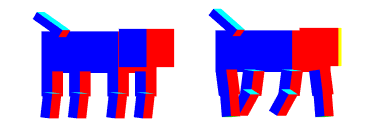
\includegraphics[scale=1]{dog}
\caption{Dog model}
\label{fig:fig1}
\end{figure}

The hierarchical model means that the parts are related to each other, starting from the torso (body), the other parts are positioned and oriented in relation to its parent. Having the following relation:

\begin{enumerate}
\item body
\begin{enumerate}
\item head
\item tail
\item left front upper leg
\begin{enumerate}
\item left front lower leg
\end{enumerate}
\item right front upper leg
\begin{enumerate}
\item right front lower leg
\end{enumerate}
\item left rear upper leg
\begin{enumerate}
\item left rear lower leg
\end{enumerate}
\item right rear upper leg
\begin{enumerate}
\item right rear lower leg
\end{enumerate}
\end{enumerate}
\end{enumerate}

\subsection {Procedural texture}
In order to add the procedural texture, the \textit{shader} and the \textit{JavaScript} were modified, in the \textit{JavaScript} file goes the code to generate the images and in the \textit{shader} the multiplication matrices between the colors and the texture presented in figure \ref{fig:fig2}.

\begin{figure}[!ht]
\centering
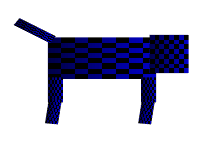
\includegraphics[scale=1]{texture}
\caption{Dog model with texture}
\label{fig:fig2}
\end{figure}

\subsection*{\textit{JavaScript}}
\begin{lstlisting}[language=JavaScript]
var texSize = 256;
var numChecks = 8;

var image1 = new Uint8Array(4*texSize*texSize);
for ( var i = 0; i < texSize; i++ ) {
    for ( var j = 0; j <texSize; j++ ) {
        var patchx = Math.floor(i/(texSize/numChecks));
        var patchy = Math.floor(j/(texSize/numChecks));
        if(patchx%2 ^ patchy%2) c = 255;
        else c = 0;
        image1[4*i*texSize+4*j] = c;
        image1[4*i*texSize+4*j+1] = c;
        image1[4*i*texSize+4*j+2] = c;
        image1[4*i*texSize+4*j+3] = 255;
    }
}

var image2 = new Uint8Array(4*texSize*texSize);
for ( var i = 0; i < texSize; i++ ) {
  for ( var j = 0; j <texSize; j++ ) {
    c = 200-j/2;
    image2[4*i*texSize+4*j] = c;
    image2[4*i*texSize+4*j+1] = c;
    image2[4*i*texSize+4*j+2] = c;
    image2[4*i*texSize+4*j+3] = 255;
  }
}
\end{lstlisting}

\subsection*{\textit{Shader}}
\begin{lstlisting}[language=HTML]
void main()
{
    gl_FragColor = fColor*(texture2D(Tex0, fTexCoord)*texture2D(Tex1, fTexCoord));
}
\end{lstlisting}

\subsection {Animation}
For the animation, all the angles movements were implemented in the render function. The head needs to turn in the direction of the viewer, all the upper and lower parts of the legs are moving, and also the tail moving up and down, trying to imitate the movement of a dog.

Also, a button is present in the screen, so the user can start and pause the walk. It is important to notice that when the user pause the walking the dog stops with all feet on the ground and not in the middle of a step.

\section{Conclusion}
After implement all the features it was possible to see the evolution of the dog as more features were being added, how to work with hierarchical models, which can be really useful when working with more complex models, implement different kinds of textures and more important, how to add animation for a model.

\end{document}